% Write the report here. You can use the nested imports via 'subimport', see the following link:
% https://www.overleaf.com/learn/latex/Management_in_a_large_project#Using_the_import_package
% You also can see an example at line n.16.

\section{Основные понятия}
Определим несколько понятий, которые понадобятся нам в дальнейшем.
\begin{definition}
    \textbf{Бид} (bid) --- это самая высокая цена, которую покупатель готов заплатить за актив. 
    Далее, бид в момент времени $t$ будет обозначаться $B_t$.
    \textbf{Аск} (ask) --- это самая низкая цена, за которую продавец готов предоставить актив. 
    Далее, аск в момент времени $t$ будет обозначаться $B_t$.
    \textbf{Бид-аск спрэд} (bid–ask spread) $s$: $s = A_t - B_t$.
    \textbf{Мид} (mid-quote price): $V_{t} = \frac{A_{t} + B_{t}}{2}$.
\end{definition}
Начнем с рассмотрения структуры лимитной книги заявок (Limit Order Book -- LOB). 
В рамках этой парадигмы организации биржевых торгов, у каждого участника есть две возможности:
\begin{itemize}
    \item выразить желание купить или продать определённое количество единиц актива по определенной цене. 
    В этом случае, биржа запомнит пару цена--количество. Множество этих пар составляет 
    лимитную книгу заявок. На рисунке \ref{LOBpic} изображено традиционное представление лимитной
    книги заявок.
    \item выразить желание купить или продать определённое количество единиц актива немедленно. 
    В этом случае он немедленно получит запрошенное количество акций (если на бирже есть необходимое количество)
    по лучшей возможной цене: к примеру, в случае покупки, если на верхнем ценовом уровне не будет достаточного
    количества единиц актива для удовлетворения заявки, то будут взяты активы из следующего ценового уровня.
    Таким образом, не гарантируется, что итоговая цена одной единицы актива будет совпадать с аском.
    
\end{itemize}

\begin{figure}
    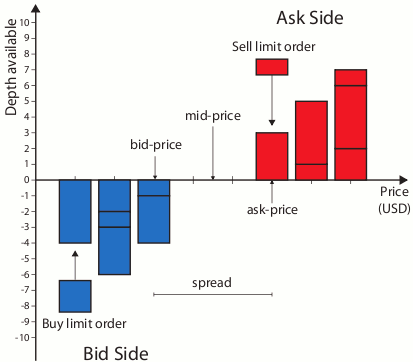
\includegraphics[scale=0.8]{fig/Graphical-representation-of-the-Limit-Order-Book.png}
    \caption{Графическое представление лимитной книги заявок}
    \label{LOBpic}
\end{figure}



Таким образом, если опустить некоторые подробности, существует два вида заявок:
\begin{definition}
    \textbf{Лимитная заявка (ордер)}(limit order) представляет собой распоряжение на покупку или продажу ценной бумаги по определенной цене или выше. 
    Этот тип заявки гарантирует цену исполнения, но не гарантирует само исполнение.
\end{definition}
\begin{definition}
    \textbf{Рыночная заявка (ордер)} (market order) представляет собой распоряжение на немедленную покупку или продажу ценной бумаги. 
    Этот тип заявки гарантирует, что она будет исполнена, но не гарантирует цену исполнения.
\end{definition}

% \begin{figure}
%     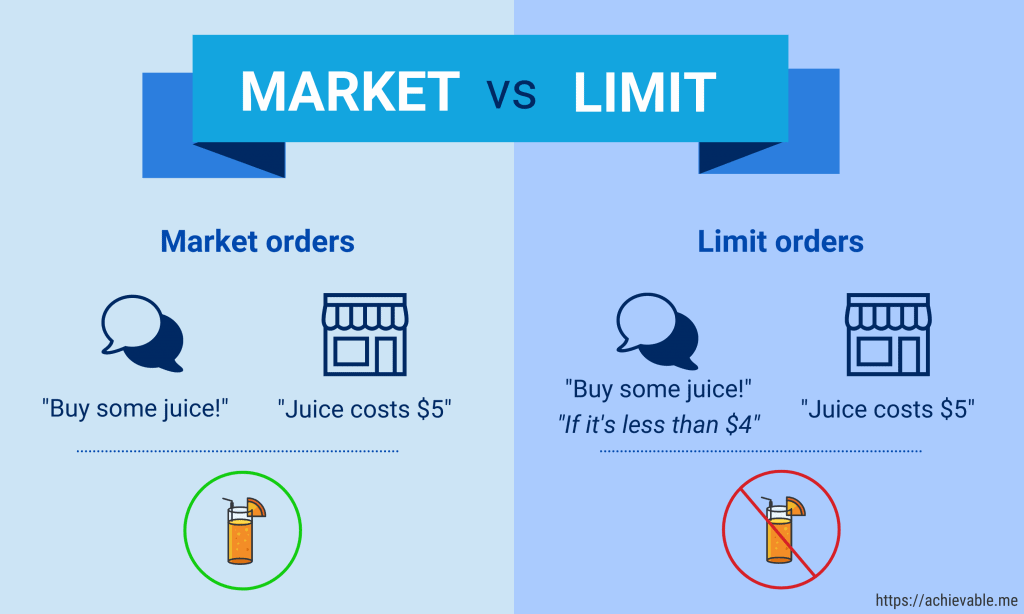
\includegraphics[scale=0.4]{fig/market-vs-limit-1024x614.png}
%     \caption{The difference between market order and limit order}
%     \label{fig:mvslim}
% \end{figure}

Теперь ясно, что если мы хотим продать или купить актив в количестве, достаточно большом, чтобы он мог оказать существенное
влияние на рынок, мы не должны делать это одной заявкой: это было бы очень дорого, поскольку крупный ордер
удалил бы все верхние уровни в лимитной книге заявок. Поэтому на практике все крупные заявки разбиваются на большое количество мелких.
Например, можно просто разделить ордер на N равных частей и продавать их через равные промежутки времени (это называется TWAP).
Но есть ли лучшее решение?


\section{Подход Обижаевой и Ванга к формализации проблемы}
В попытке найти лучшее решение, мы рассматриваем модель Обижаевой--Ванга,
в терминах которой задача имеет следующий вид: \par
\begin{align*} \label{oEproblem}
    J_0 &= \min _{\{x_0 \cdots x_N \}} E_0 \left[ \sum _{n=0}^N [A_{t_n} + x_n /(2q)] x_n\right],  \\
    A_{t_n} &= F_{t_n} + \lambda (X_0 - X_{t_n}) + s/2 + \sum _{i=0}^{n-1} x_i \kappa e^{- \rho \tau (n - i)},
 \end{align*}
 
где
\begin{itemize}
 \item трейдер должен купить $\mathbf{X_0}$ единиц актива за фиксированный период времени $[0,T]$;
 \item $x_{t_n}$ размер оредра в момент времени $t_n = \tau n$ (здесь, $\tau = T / N$); 
 \item $X_{t_n} := X_0 - \sum _{t_k < t_n} x_{t_k}$;
 \item $B_{t_n}$ и $A_{t_n}$ --- бид и аск в момент времени $t_n$; 
 \item $V_{t_n} = \frac{A_{t_n} + B_{t_n}}{2}$ --- мид; 
 \item $s$ --- бид-аск спрэд;
 \item $F_t$ --- фундаментальная (справедливая) цена актива;
 \item $q(P)$ распределение лимитной книги заявок $P$ (по ценам $[a, b]$ доступно $\int_a^b q(p) dP$ единиц актива);
 % \item $q$, $\lambda$ and $\rho$ is a LOB density, the permanent price impact and the resiliency.
 \item параметр $\lambda$ --- постоянный маркет импакт (справдливая цена $V_t$ в результате исполнения ордера объема $x$ меняется по закону: $V_{t+} = V_t + \lambda x$);
  \item $\kappa = \frac{1}{q} - \lambda $;
 \item параметр $\rho$ --- упргуость стакана (resiliency).
\end{itemize}

Данная задача была решена в статье \cite{obizhaeva2013optimal}:
\begin{theorem}
    Решение задачи оптимального исполнения:
    \begin{multline*}
        x_n = - \frac{1}{2} \delta_{n + 1} [D_{t_n} (1 - \beta_{n + 1} e^{ - \rho \tau} + 2 \kappa \gamma_{n+1} e^{ - 2 \rho \tau}) 
         - X_{t_n} (\lambda + 2 \alpha_{n+1} - \beta_{n+1}\kappa e^{ - \rho \tau}) ], 
    \end{multline*}
    где $x_N = X_N$ и $D_t = A_t - V_t - s/2$. Ожидаемая цена будущих сделок в рамках
    стратегии оптимального исполнения меняется по закону
    \begin{equation*}
        J_{t_n} = (F_{t_n} + s/2) X_{t_n} + \lambda X_0 X_{t_n} + \alpha_n X_{t_n} ^2 + \beta_{n} D_{t_n} X_{t_n} + \gamma_n D_{t_n}^2, 
    \end{equation*}
    где коэффициенты $\alpha_{n+1}$, $\beta_{n+1}$, $\gamma_{n+1}$ и $\delta_{n+1}$ определяются рекурснивно по формулам:
    \begin{equation*}
        \alpha_{n} = \alpha_{n+1} - \frac{1}{4} \delta _{n+1} (\lambda + 2 \alpha_{n+1} - \beta_{n+1} \kappa e^{- \rho \tau})^2, 
    \end{equation*}
    \begin{multline*}
        \beta_{n} =  \beta_{n+1} e^{- \rho \tau} + \frac{1}{2} \delta _{n+1} (1 - \beta_{n+1} e^{- \rho \tau} 
         + 2 \kappa \gamma_{n+1} e^{- 2 \rho \tau}) (\lambda + 2 \alpha_{n+1} - \beta_{n+1} \kappa e^{-\rho \tau}), 
    \end{multline*}
    \begin{equation*}
         \gamma_n =   \gamma_{n+1} e^{- 2 \rho \tau} - \frac{1}{4} \delta _{n+1} (1 - \beta _{n+1} e^{- \rho \tau} 
    + 2 \gamma _{n+1} \kappa e^{- 2 \rho \tau})^2, 
    \end{equation*}
    где $\delta_{n+1} = [1/(2q) + \alpha_{n+1} - \beta_{n+1} \kappa e^{-\rho \tau} + \gamma _{n+1} \kappa ^2 e^{- 2 \rho \tau}]^{-1}$ и начальные условия
    \begin{equation*}
        \alpha_{N} = 1/(2q) - \lambda, \;\;\;\;\;\;\; \beta_N = 1, \;\;\;\;\;\;\; \gamma_N = 0.
    \end{equation*}
\end{theorem}

В нашем исследовании мы будем рассматривать предел этого решения.

\begin{theorem} \label{OEmainformula}
    При $N \rightarrow \infty$, стратегия оптимального исполнения принимает вид:
    \begin{align*}
        & \lim _{N \rightarrow \infty} x_0 = x_{t = 0} = \frac{X_0}{\rho T + 2}, \\
        & \lim _{N \rightarrow \infty} x_n / (T/N) = \dot X _t = \frac{\rho X_0}{\rho T + 2}, \;\;\;\;\;\; t \in (0, T), \\
        & \lim _{N \rightarrow \infty} x_0 = x_{t = 0} = \lim _{N \rightarrow \infty} x_n / (T/N) = x_{t=T}=  \frac{X_0}{\rho T + 2}.  %\\
    \end{align*}
    где $x_0$ первая сделка за отведенный период, $x_N$ --- последняя, и $\dot X _t$ скорость трейдинга между ними.
\end{theorem}

Таким образом, мы имеем явную формулу для стратегии оптимального исполнения. Но нам необходимо каким-либо образом найти
параметр $\rho$ для того, чтобы применить её на практике. \par

Другое возможное приложение параметра $\rho$ даёт формула, определяющая динамику аска после исполнения ордера глубины $x$:
\begin{equation*}
        A_t = \overline p _t + \frac{s}{2} + x \kappa e^{- \rho t}.
\end{equation*}
Поскольку, к примеру, на московской бирже, минимальный шаг цены составляет, в основном, около $0.05\%$ 
от спотовой цены (см. \ref{price_step}), согласно модели стакан будет полностью восстанавливаться 
после исполнения "большого" ордера (для которого $x \kappa \approx 0.01 * A_t $) примерно за $t = \frac{10}{\rho}$.
\begin{figure}
    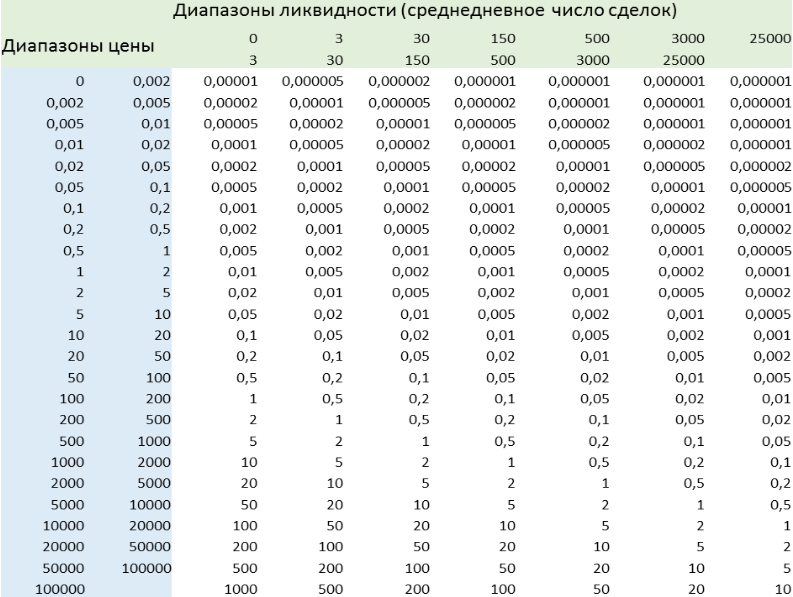
\includegraphics[scale=0.64]{fig/price_step.png}
    \caption{Правила определения расчетного шага цены (сайт московской биржи).}
    \label{price_step}
\end{figure}

\section{Как подобрать $\rho$?}
Предлагаемая нами методология основана на следующей теореме.
\begin{theorem}\label{lilreg}
    Для упрощения записей введём обозначения:
    \[
    \Delta t_{k} := t_{k} - t_{k-1}, \; \; \; \;   
    \Delta A_{k} := A_{k} - A_{k-1}. 
    \]
    В регрессии                                                                                                                                                                                                                                                                                                                                                                                       
    \begin{equation*}
            \frac{\Delta A_{k+1}}{\Delta t_{k+1}} - \frac{\Delta A_{k}}{\Delta t_{k}}
            = -B \Delta A_k + B (\lambda + \kappa) x_{t_k} - B \kappa x_{t_{k+1}} + 
            (\lambda + \kappa) \left(\frac{x_{t_{k+1}}}{\Delta t_{k+1}} - \frac{x_{t_k}}{\Delta t_{k}}\right),
    \end{equation*}
    где $x_{t_k}$ и $A_{t_k}$ --- глубина ордера и аск в момент времени $t_k$, соответственно, \\
    $\rho = B + O(\rho^2 \Delta t)$ .
\end{theorem}
Таким образом, мы прадлагаем следующий эмпирический путь подбора параметра $\rho$:
\begin{enumerate}
    \item Подготавливаем и очищаем данные, проверяем их на соответствие модели Обижаевой--Ванга.
    \item Оцениваем по данным регрессию
    \begin{equation*}
        \frac{\Delta A_{k+1}}{\Delta t_{k+1}} - \frac{\Delta A_{k}}{\Delta t_{k}}
            = -B \Delta A_k + B (\lambda + \kappa) x_{t_k} - B \kappa x_{t_{k+1}} + 
            (\lambda + \kappa) \left(\frac{x_{t_{k+1}}}{\Delta t_{k+1}} - \frac{x_{t_k}}{\Delta t_{k}}\right),
    \end{equation*} 
    где
    \begin{itemize}
        \item $\Delta A_{k}$ изменение аска в следствие исполнения заявки размера $x_k$ в момент времени $t_k$.
        \item $\Delta t_{k}$ время между $k$ и $k + 1$ заявками.
    \end{itemize}
    \item Если $\rho^2 \Delta t$ мало, то считаем, что $B \approx \rho$ и исполняем заявку в соответствии с \eqref{OEmainformula}.
\end{enumerate}
Если последнее условие не выполнено, то можно попытаться применить подход, изложенный в приложении \ref{AppendixBigRho}.
Однако, если мы решаем практическую задачу оптимального исполнения заявки за, например, $10$ минут, то при $\rho > 0.5$ 
в соответствии с формулой \eqref{OEmainformula} получаем, что, de facto, модель рекомендует продать менее, чем $\approx 0.3\%$ объема
ордера за первую и последнюю сделки, а остальное равномерно продавать внутри врменного промежутка, что практически мало отличимо от 
алгоритма TWAP. 
\par
Таким образом, мы считаем, что наш подход при всей простоте, полностью описывает алгоритм практической торговли. 


\section{Данные}
\subsection{Источники и предобработка}
Мы работали с ордерлогами (\href{https://fs.moex.com/f/3198/specifikacija-formata-dannyh.pdf}{спецификация}). Было написано несколько 
\href{https://github.com/VsevolodZaostrovsky/OWModel/tree/main/New%20data/data%20preparing}{программ},
которые, в совокупности, распаршивали исходные записи в таблицу из четвёрок (время, аск до исполнения ордера, аск после исполнения ордера, глубина ордера). 
Следует обратить внимание на то, что заявки, поглощающие несколько уровней, представляются в данных в виде последовательности заявок, поэтому 
перед началом обработки их следует объединить: объем ордера есть сумма объемов, аск до исполнения --- аск до исполнения первого ордера,
аск после исполнения --- аск после исполнения последнего ордера. Фрагмент таблицы, на котором представлен фрагмент обработанных данных
и схематичное изображение изложенной выше операции, изображен на рисунке \ref{datacsv}.
 Рассматривались данные за 
03.03.2021 (середина недели, месяц максимально удаленный от праздников, 
год, удаленный от начала СВО и начала эпидемии COVID.)
\begin{figure}
    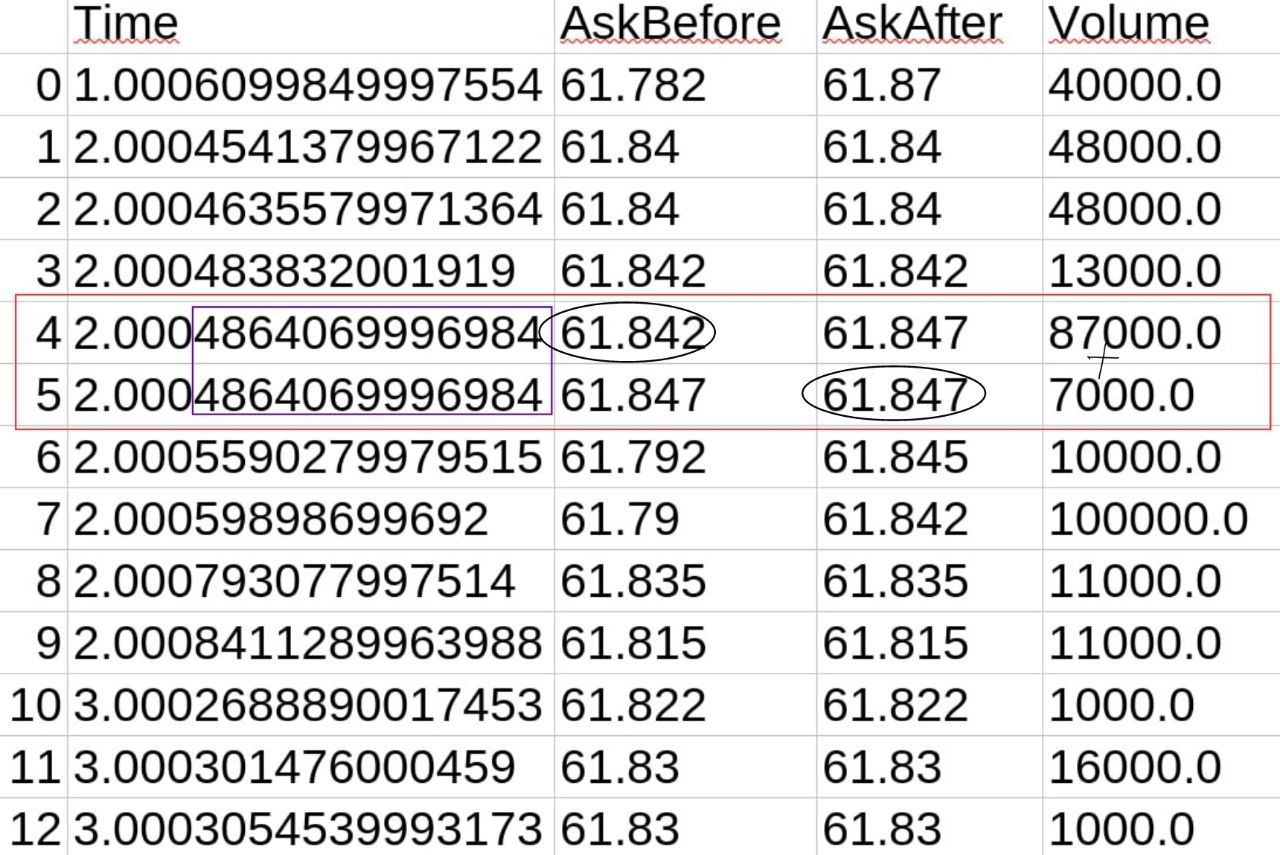
\includegraphics[scale=0.35]{fig/datscsv.jpg}
    \caption{Данные после первого этапа парсинга}
    \label{datacsv}
\end{figure}

\subsection{Выбор инструмента и начальный анализ данных} \label{InitAnal}
В целом, известно, что российский рынок характеризуется низким уровнем ликвидности и низкой интенсивностью торгов. 
Для подбора параметров и статистических исследовании
нам нужно относительно большое количество данных, по этой причине
для очень существенной части активов, торгуемых на московской бирже, 
исследование в духе нашего было бы невозможно: даже в категориях 
активов, считающихся ликвидными,
встречается немало инструментов \footnote{Даже среди валютных пар большая 
часть имеет очень низкую интенсивность торгов, например, CHFRUB\_TOM, HKDRUB\_TOM, 
JPYRUB\_TOM, KZTRUB\_TOM.}, по которым совершается порядка нескольких десятков сделок в день (и даже меньше). 
Поэтому мы решили рассмотреть две категории активов: самые ликвидные валютные пары
и несколько наиболее ликвидных акций (мы исключили из рассмотрения акции ВТБ, поскольку их сильное дробление создаёт 
численные проблемы).
\par
При этом, почти у всех активов подавляющее большинство сделок не поглащает ни одного уровня 
(те фактическая цена совершения сделки равна аску, см. таблицы \ref{tableanalCUnew} и \ref{tableanalSE}). 
\par
Заметим, что при изучении данных мы подтвердили широко известную закономерность: 
распределение времени между сделками очень похоже для всех активов и напоминает экспоненциальное 
(см. \ref{timedistr}).


\subsection{Спайки}

Данные характеризуются очень большим числом количеством резких и коротких скачков аска. 
Пересечение множеств
сотни самых больших сделок и сотни сделок, сдвинувших аск сильнее всего, пусто. Таким образом, похоже, что ордеров,
которые существенно двигают аск за счёт своего размера на рынке мало, то есть цена двигается, в основнов, по фундаментальным причинам.
На наш взгляд, такая структура данных может послужить основанием для того, чтобы усомниться в валидности модели Обижавеой--Ванга 
для российских данных, однако и не дает возможности с уверенносью сказать, что модель не применима. 
\par
Откуда же берутся эти скачки и что они из себя представляют? В стакане в каждый момент времени поддерживается тонкий баланс, любой
маленький ордер, более выгодный, чем лучшая цена, будет почти мгновенно поглощён рынком. Конечно, если возникает необходимость в продаже
или покуке небольшого количетсва актива, этим разумно воспользоваться.

\begin{example}
    Пусть аск равен $10$, а бид --- $9$. Если мы хотим продать небольшое количество актива, то можно, например, разместись ордер
    на продажу актива по цене $9.1$, тогда пока ордер не будет исполнен, аск станет равным $9.1$, однако, скорее всего, лот очень
    быстро выкупят, поскольку он намного лучше аска и даже мида. Таким образом, мы продадим актив по цене $9.1$ вместо $9$, 
    расплатившись за это довольно несущественным риском.
\end{example}

Мы проанализировали несколько конкретных спайков в ручную и оказалось, что происходит именно то, что описано в примере. 
Ясно, что эти скачки, в целом, не характеризуют
динамику рискового актива, поэтому целесообразно исключить их из исследуемого датасета. \par


\subimport{./tab/}{table1.tex}


% В паре ликвидных валют EURUSD000TOM происходит лишь порядка пятисот сделок в день. Тем не менее, мы решили исследовать и эту пару,
% поскольу данных (если не слишком сильно их фильтровать) достаточно для обучения модели, в то же время, характер торгов, очевидно,
% другой. \par
% Таким образом, мы решили остановить свой выбор на парах
% USD000UTSTOM и EURUSD000TOM.

\section{Результаты регрессий} \label{rowregr}

\subsection{Регрессионное уравнение на данных}
\par
В терминах нашего датасета (см. вид данных на \ref{datacsv}), регрессия на $B$ выглядят следующим образом:
\begin{align*}
\frac{\textrm{AskAfter}(k+1) - \textrm{AskBefore}(k+1)}{\textrm{Time}(k+2) - \textrm{Time}(k+1)} 
- \frac{\textrm{AskAfter}(k) - \textrm{AskBefore}(k)}{\textrm{Time}(k+1) - \textrm{Time}(k)}
= \\ 
= -B (\textrm{AskAfter}(k) - \textrm{AskBefore}(k)) + B (\lambda + \kappa) \textrm{Volume}(k) 
- B \kappa \textrm{Volume}(k+1) + \\
+ (\lambda + \kappa) \left(\frac{\textrm{Volume}(k+1)}{\textrm{Time}(k+2) - \textrm{Time}(k+1)} 
- \frac{\textrm{Volume}(k)}{\textrm{Time}(k+1) - \textrm{Time}(k)}\right).
\end{align*}
Фактически, это просто формула \eqref{lilreg}, где мы полагаем:
\begin{itemize}
    \item $\Delta A_{k} = \textrm{AskAfter}(k) - \textrm{AskBefore}(k)$, а $x_k = \textrm{Volume}(k)$,
    \item $\Delta t_{k} = \textrm{Time}(k+1) - \textrm{Time}(k)$.
\end{itemize}
\par

\subsection{Результаты регрессий на неагрегированных данных}
Как видно из таблицы \ref{liqmetrics}, разные метрики ликвидности довольно сильно кореллированы друг с другом, поэтому 
мы решили выводить лишь одну из них, чтобы не загромождать таблицу.
\par
\subimport{./tab/}{LiqMetrics.tex}

\subimport{./tab/Appendix/}{RD_CU.tex}

\subimport{./tab/Appendix/}{RD_SE.tex}


В данном случае нет формальных оснований полагать, что полученные числа 
(таблицы \ref{RD_CU_1}--\ref{RD_SE_2}) имеют какое бы то ни было отношение к модели 
Обижаевой--Ванга. Особой связи с ликвидностью тоже не прослеживаются. Мы считаем, что это связано с тем, 
что в данной ситуации $B$ слишком велико и модель искажается достаточно сильно для того, 
чтобы экономический смысл коэффициентов изменился. Тем не менее отсюда можно извлечь содержательный вывод:
модель считает рынок достаточно ликвидным, чтобы оптимальным решением был TWAP. 
Отметим, что, возможно, развитие идей, высказанных в разделе \ref{AppendixBigRho}, 
помогло бы установить точную связь между вычисленным в регрессии
коэффициентом $B$ и теоретическим $\rho$. 


\subsection{Результаты регрессий на агрегированных данных}
Мы обнаружили, что на сырых данных $\rho$ получается очень большим (см. \ref{rowregr}). Поэтому мы тестировали разные
варианты агрегации данных: иными словами, объединяли мелкие ордера в более крупные в попытках сформировать ситуацию,
более близкую к предположениям модели Обижаевой--Ванга. Следующие результаты были получены на датасете, в котором мы 
записывали аск в начале и в конце скунды, а за объем оредра считали общий объем сделок за секунду.
\par
Для $B ^*$ всё аналогично, но меняется методология рассчёта аска. Теперь это не лучшая цена покупки
одной единицы актива, а лучшая цена покупки миллиона единиц актива. \par

\subimport{./tab/}{AggregatedDS_SE.tex}

Как видно, для валют абсолютно чётко прослеживается связь между разными метриками ликвидности и $B$,
что даёт основания считать вычисленный коэффициент валидной мерой ликвидности актива. Кроме того, 
во всех случаях $B$ довольно мал по модулю, так что можно считать, что $B = \rho$. Этого достаточно,
чтобы практически осуществить оптимальное исполнение в соответствии с моделью Обижаевой--Ванга.
Последние две валютных пары существенно выбиваются из общей колеи. Однако в их случае выборки ничтожно малы,
так что, вероятно, методика просто напросто "переобучилась".
\par
\subimport{./tab/}{AggregatedDS_SE.tex}
У акций также есть чёткая связь между разными метриками ликвидности и $B$,
что даёт основания считать вычисленный коэффициент валидной мерой ликвидности актива. Кроме того, 
во всех случаях $B$ довольно мал по модулю, так что можно считать, что $B = \rho$. Этого достаточно,
чтобы практически осуществить оптимальное исполнение в соответствии с моделью Обижаевой--Ванга.
\par
Стоит отметить, что эти выводы, при всей привлекательности, не робастны по отношению к изменению промежутка 
агрегации. 
\par
Данные при таком подходе очень сильно отфильтрованы и нетривиальным является вопрос того,
репрезентуют ли они после всех изменений экономику рынка. Результаты на неагрегированных 
данных оказались совсем другими, так что, вероятнее всего, ответ отрицательный.



